\RequirePackage{luatex85}
\documentclass{standalone}
%\url{https://tex.stackexchange.com/q/312405/86}
\usepackage{tikz}
\usetikzlibrary{tqft}

\begin{document}
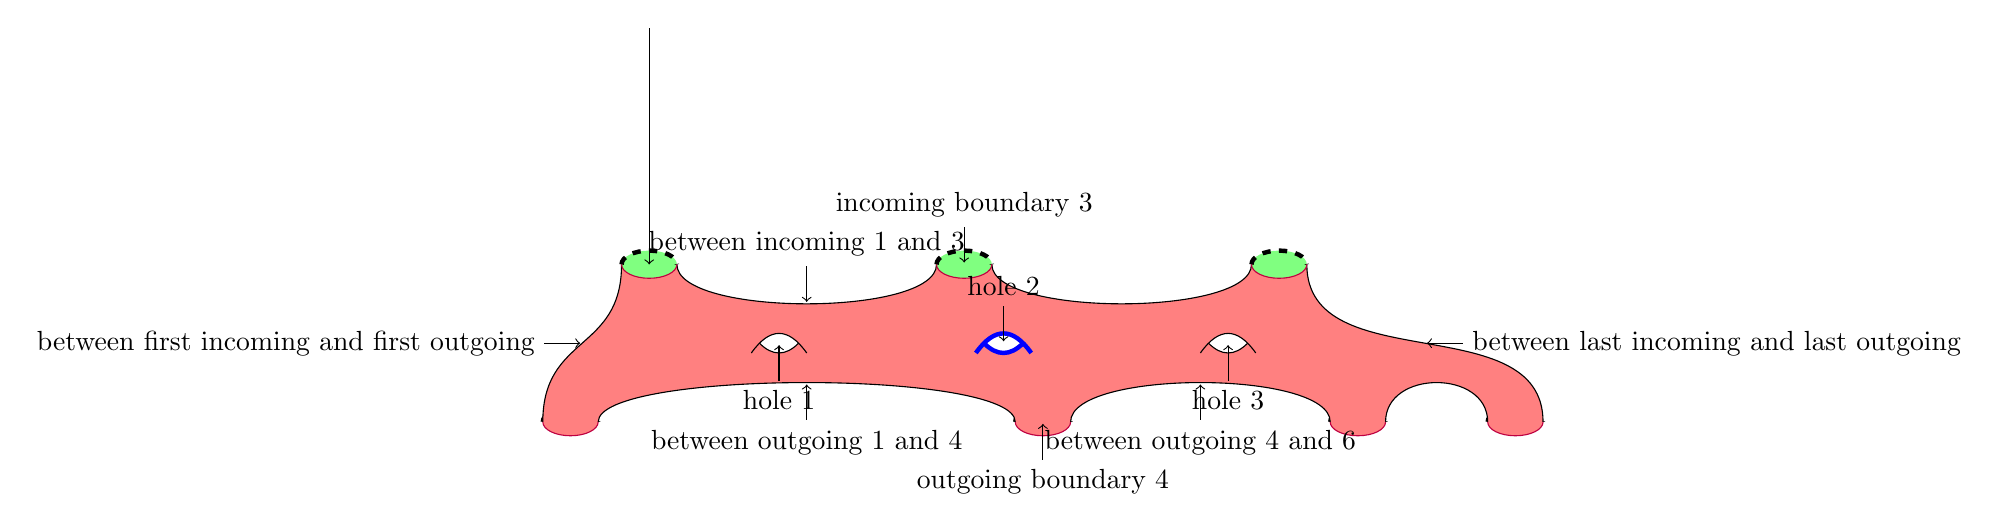
\begin{tikzpicture}[
  tqft,
  every outgoing boundary component/.style={fill=blue!50},
  outgoing boundary component 3/.style={fill=none,draw=red},
  every incoming boundary component/.style={fill=green!50},
  every lower boundary component/.style={draw,ultra thick, dashed},
  every upper boundary component/.style={draw,purple},
  cobordism/.style={fill=red!50},
  cobordism edge/.style={draw},
  genus=3,
  hole 2/.style={ultra thick, blue},
  view from=incoming,
  anchor=between incoming 1 and 2
]
\pic[name=a,tqft,incoming boundary components=5,skip incoming boundary components={2,4},outgoing boundary components=7,skip outgoing boundary components={2,3,5},offset=-.5];

\begin{scope}[every pin edge/.style={<-}]
\foreach \anchor/\ang in {
  hole 1/-90,
  hole 2/90,
  hole 3/-90,
  incoming boundary 3/90,
  outgoing boundary 4/-90,
  between last incoming and last outgoing/0,
  between first incoming and first outgoing/180,
  between incoming 1 and 3/90,
  between outgoing 1 and 4/-90,
  between outgoing 4 and 6/-90
} {
  \node[pin=\ang:\anchor,at=(a-\anchor),inner sep=0pt] {};
}
\draw[<-] (0,0) -- ++(0,3);
\end{scope}
\end{tikzpicture}
\end{document}
